\documentclass[tikz]{standalone}
\usepackage{tikz}
\usetikzlibrary{positioning}


\begin{document}

\newcommand{\cost}{c}
\newcommand{\lightred}{white!60!red}
\newcommand{\partfrac}[2]{\frac{\partial #1}{\partial #2}}
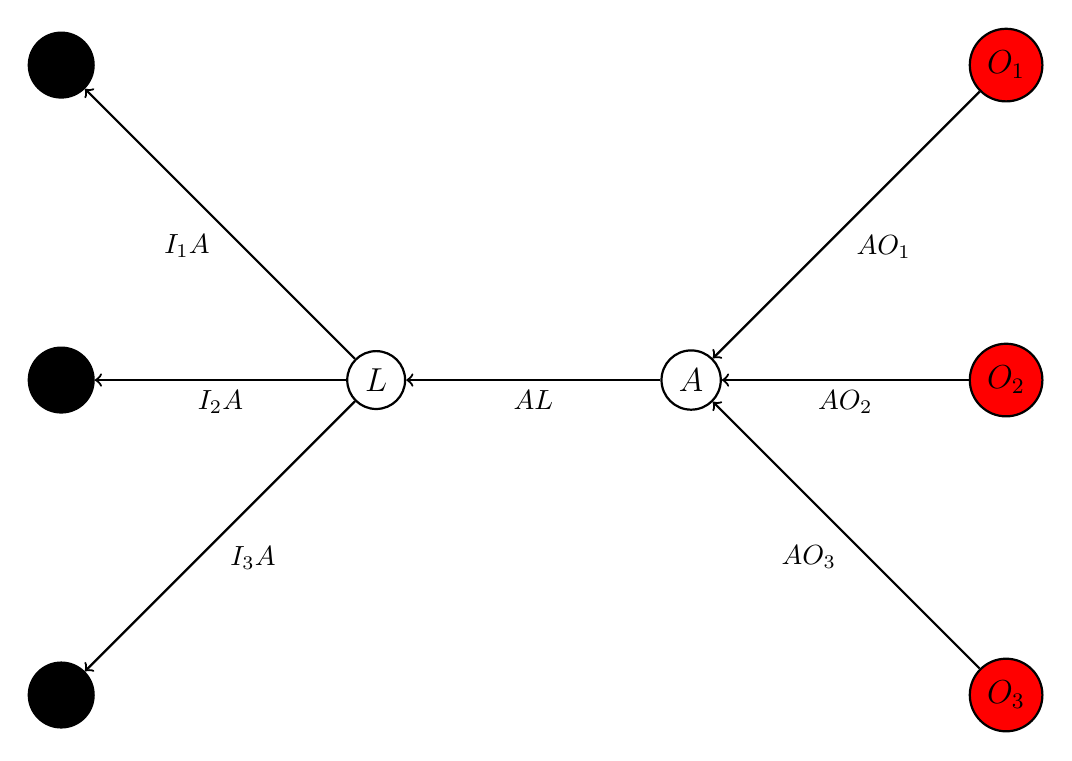
\begin{tikzpicture}[auto, node distance=4cm, every loop/.style={},
thick,main node/.style={circle,draw,font=\sffamily\large\bfseries}]

\node[main node] [fill=\lightred] (A) {$\partfrac{I_1}{\cost}$};
\node[main node] [fill=\lightred] (B) [below of=A] {$\partfrac{I_2}{\cost}$};
\node[main node] [fill=\lightred] (C) [below of=B] {$\partfrac{I_3}{\cost}$};
\node[main node] (D) [right of=B]  {$\partfrac{L}{\cost}$};
\node[main node] (P) [right of=D]   {$\partfrac{A}{\cost}$};
\node[main node] [fill=red] (E) [right of=P] {$\partfrac{O_2}{\cost}$};
\node[main node] [fill=red] (F) [below of=E] {$\partfrac{O_3}{\cost}$};
\node[main node] [fill=red] (G) [above of=E]  {$\partfrac{O_1}{\cost}$};;

\path[every node/.style={font=\sffamily\normalsize}]
(D) [->] edge node [] {$\partfrac{I_1}{A}$} (A)
(D) [->] edge node [] {$\partfrac{I_2}{A}$} (B)
(D) [->] edge node [] {$\partfrac{I_3}{A}$} (C)
(P) [->] edge node [] {$\partfrac{A}{L}$} (D)
(E) [->] edge node [] {$\partfrac{A}{O_2}$} (P)
(F) [->] edge node  {$\partfrac{A}{O_3}$} (P)
(G) [->] edge node  {$\partfrac{A}{O_1}$} (P);
\end{tikzpicture}

\end{document}